
\documentclass[11pt, a4paper]{article}
\usepackage[utf8]{inputenc}
\usepackage{amsmath, amssymb, amsthm}
\usepackage{geometry}
\usepackage{xcolor}
\usepackage{hyperref}
\usepackage{parskip}
\usepackage{tikz} % Required for drawing diagrams
\usetikzlibrary{arrows.meta, positioning, calc}
\usepackage{caption}
\usepackage{parskip}

% --- Custom Environments for Pedagogy ---
\usepackage{tcolorbox} % For highlighting key insights
\newtcolorbox{insight}{
    colback=gray!10,
    colframe=black,
    title=\textbf{Pedagogical Insight},
    fonttitle=\bfseries
}

% Geometry settings
\geometry{margin=1in}

% Theorem environments
\newtheorem{definition}{Definition}
\newtheorem{theorem}{Theorem}
\newtheorem{example}{Example}
\newtheorem{remark}{Remark}

% Custom commands
\newcommand{\Q}{\mathbb{Q}}
\newcommand{\Z}{\mathbb{Z}}
\newcommand{\C}{\mathbb{C}}
\newcommand{\Gal}{\text{Gal}}

\title{\textbf{An Introduction to Galois Theory}\\ \large Symmetries of Equations and Field Extensions \\
and Connections with Algorithmic Agent Theory \\
BCOM WP0052 (LU003)}
\author{Pedagogical Series (Giulio Ruffini\footnote{giulio.ruffini@bcom.one} with Gemini-Gaia)}
\date{Feb 1 2026}

\begin{document}

\maketitle
 
\begin{abstract}
    This note aims to demystify Galois Theory by connecting its foundational definitions to a broader principle of \textit{computational tractability}. We begin with the elementary example of $\mathbb{Q}(i)$ to illustrate how algebraic symmetries arise from the indistinguishability of roots. We then proceed to the heart of the theory: the rigorous link between symmetry and solvability.
    We reframe the Abel-Ruffini theorem not merely as a limit on polynomials, but as a positive definition of structure: a problem is "solvable" if and only if its symmetry group is \textit{compositional} (decomposable into abelian steps). When this condition fails—as with the monolithic $A_5$ group—we show that progress requires the discovery of new atomic primitives (the ``Nuclear Option"). Finally, we discuss this logic in the context of the continuous domain (Lie Theory) and Artificial Intelligence. Drawing on Poggio’s work on compositionality and Kolmogorov Theory, we demonstrate that ``learning" is the algorithmic cycle of discovering these symmetries. The resulting ``staircase" in the Kolmogorov Structure Function reveals that intelligence is the interplay of two modes: \textbf{exploiting} existing tools through composition, and \textbf{inventing} new cognitive cores to further compositionally compress the ``unsolvable".
\end{abstract}

\clearpage


\tableofcontents
\clearpage

%%%%%%%%%%%%%%%%%%%%%%%%%%%%%%%%%%%%%%%%%%%%%%%%%%%
\part{The Foundations of Algebraic Symmetry }

\section{The ``Hello World'' of Galois Theory: $\Q(i)$}

Galois theory represents a shift in perspective. In elementary algebra, we ask: \textit{``What are the numbers that solve this equation?''} In Galois theory, we ask: \textit{``How symmetric is the set of solutions? Can we swap them without breaking the arithmetic?''}

Unlike geometric symmetry, which deals with shapes in space, Galois symmetry deals with the algebraic structure of numbers. To make this precise, we define our stage using two fields:
\begin{enumerate}
    \item The \textbf{Base Field} $F = \Q$ (the rational numbers).
    \item The \textbf{Extension Field} $K = \Q(i)$, constructed by adjoining a root of $x^2 + 1 = 0$ to $\Q$. Elements in $K$ are of the form $a + bi$, where $a, b \in \Q$.
\end{enumerate}

\subsection{The Definition of a Symmetry (Automorphism)}

We do not simply swap roots. We look for a structural transformation of the entire field.

\begin{definition}[Field Automorphism]
    An automorphism of an extension $K/\Q$ is a bijective map $\sigma: K \to K$ such that:
    \begin{enumerate}
        \item \textbf{Structure Preservation:} For all $\alpha, \beta \in K$:
        \[ \sigma(\alpha + \beta) = \sigma(\alpha) + \sigma(\beta) \quad \text{and} \quad \sigma(\alpha \cdot \beta) = \sigma(\alpha) \cdot \sigma(\beta) \]
        \item \textbf{Base Fixing:} For all $q \in \Q$, $\sigma(q) = q$.
    \end{enumerate}
\end{definition}


\subsection{Locating the Automorphisms}
Since every element in $\Q(i)$ looks like $a + bi$, and $\sigma$ fixes $a$ and $b$ (because they are rational), the action of $\sigma$ is entirely determined by $\sigma(i)$.

Where can $i$ go? We use the fundamental equation:
\[ i^2 = -1 \]
Apply $\sigma$ to both sides:
\[ \sigma(i^2) = \sigma(-1) \]
Using the homomorphism property and the fact that $-1 \in \Q$:
\[ \sigma(i) \cdot \sigma(i) = -1 \]
\[ (\sigma(i))^2 = -1 \]

\textbf{The Crucial Insight:} $\sigma(i)$ must be a number in our field that \textit{also} squares to $-1$. The roots of $x^2+1$ are $\{i, -i\}$. Thus, there are exactly two possibilities:
\begin{itemize}
    \item \textbf{Case 1 (Identity):} $\sigma(i) = i$. This fixes every element.
    \item \textbf{Case 2 (Conjugation):} $\sigma(i) = -i$. This maps $a+bi \mapsto a-bi$.
\end{itemize}

\begin{center}
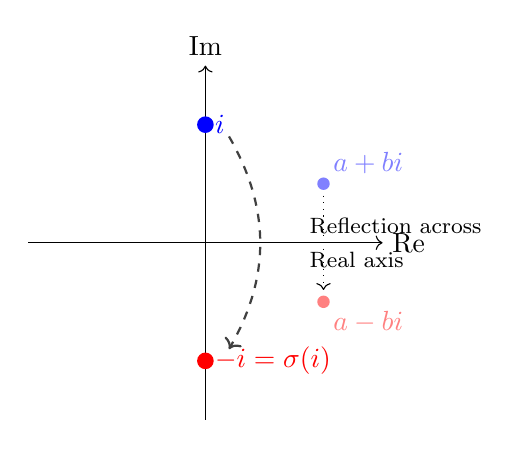
\begin{tikzpicture}[scale=1.5]
    % Axes
    \draw[->] (-1.5,0) -- (1.5,0) node[right] {Re};
    \draw[->] (0,-1.5) -- (0,1.5) node[above] {Im};
    
    % Points
    \fill[blue] (0,1) circle (2pt) node[right] {$i$};
    \fill[red] (0,-1) circle (2pt) node[right] {$-i = \sigma(i)$};
    
    % Reflection Arrow
    \draw[->, dashed, thick, darkgray] (0.2, 0.9) to[bend left] (0.2, -0.9);
    \node at (0.8, 0) [right, align=left] {\footnotesize Reflection across\\ \footnotesize Real axis};
    
    % Generic point
    \fill[blue!50] (1,0.5) circle (1.5pt) node[above right] {$a+bi$};
    \fill[red!50] (1,-0.5) circle (1.5pt) node[below right] {$a-bi$};
    \draw[->, dotted] (1, 0.4) -- (1, -0.4);

\end{tikzpicture}
\captionof{figure}{Visualizing the Automorphism $\sigma(z) = \bar{z}$. Note that the Real axis (Rational numbers) remains fixed, while the Imaginary component flips.}
\end{center}

\subsection{The ``Magic'' of Consistency}
Why is the map $\sigma(i) = -i$ allowed? Does it break the algebra?
Consider the defining relation $i \cdot i = -1$. If we swap $i$ for $-i$, we must ensure the equation still holds.

\begin{center}
\fbox{
\begin{minipage}{0.8\textwidth}
\textbf{Checking the Algebraic "Magic":} \\
We replace $i$ with $-i$. Does the multiplication law hold?
\[ (-i) \cdot (-i) = (-1)(-1)(i \cdot i) = 1 \cdot (-1) = -1 \]
\end{minipage}
}
\end{center}

The swap works precisely because the destination root ($-i$) obeys the same algebraic laws as the source root ($i$). They are "algebraic twins."


\section{The ``Cascade'' of Automorphisms}

A field automorphism is often defined on an infinite set of numbers. However, we do not need to define the mapping for every single number individually. 

\begin{theorem}[Determination by Generators]
    Let $K = \Q(\alpha_1, \dots, \alpha_n)$ be a field extension generated by elements $\alpha_i$. An automorphism $\sigma: K \to K$ fixing $\Q$ is completely determined by the values $\sigma(\alpha_1), \dots, \sigma(\alpha_n)$.
\end{theorem}

\subsection{Proof of the Cascade}
Any element $\gamma \in K$ can be written as a polynomial in the generators with rational coefficients:
\[ \gamma = \sum_{k} c_k (\alpha_1)^{p_1} \dots (\alpha_n)^{p_n} \]
where $c_k \in \Q$.

Applying $\sigma$ to $\gamma$, we use the properties of homomorphism (preservation of $+$ and $\times$) to propagate the map down to the generators:

\begin{align*}
    \sigma(\gamma) &= \sigma\left( \sum_{k} c_k (\alpha_1)^{p_1} \dots (\alpha_n)^{p_n} \right) \\
    &= \sum_{k} \sigma(c_k \cdot (\alpha_1)^{p_1} \dots (\alpha_n)^{p_n}) & (\text{Preservation of Sums}) \\
    &= \sum_{k} \sigma(c_k) \cdot \sigma(\alpha_1)^{p_1} \dots \sigma(\alpha_n)^{p_n} & (\text{Preservation of Products}) \\
    &= \sum_{k} c_k \cdot (\sigma(\alpha_1))^{p_1} \dots (\sigma(\alpha_n))^{p_n} & (\text{Fixing Base Field } \Q)
\end{align*}

\textbf{Conclusion:} The final expression depends \textit{only} on the values of $\sigma(\alpha_i)$. Once the action on the generators is chosen, the action on the entire field is fixed.


\subsection{Algebraic Indistinguishability}
The existence of the automorphism $\sigma(i) = -i$ proves a profound fact about the rational numbers.

\begin{theorem}[Indistinguishability]
    Let $P(x)$ be any polynomial with coefficients in $\Q$. If $P(i) = 0$, then $P(-i) = 0$.
\end{theorem}

\begin{proof}
    Let $P(x) = \sum c_k x^k$ with $c_k \in \Q$. If $P(i) = 0$, apply $\sigma$:
    \[ \sigma\left( \sum c_k i^k \right) = \sigma(0) \]
    Since $\sigma$ fixes $\Q$ and respects powers:
    \[ \sum c_k (\sigma(i))^k = 0 \implies \sum c_k (-i)^k = 0 \implies P(-i) = 0 \]
\end{proof}

There is no algebraic test using rational coefficients that can distinguish $i$ from $-i$.


\subsection{The Counter-Example Analysis}
Consider the polynomial proposed in the discussion:
\[ P(x) = x^3 + i \]
We observe that $i$ is a root: $i^3 + i = -i + i = 0$.
However, if we test $-i$:
\[ P(-i) = (-i)^3 + i = i + i = 2i \neq 0 \]
\textbf{Why did the theorem fail?}
The theorem requires the coefficients of $P(x)$ to be in the base field $\Q$.
Your polynomial has a coefficient $i$, which is in the extension field, not the base field.
\[ i \notin \Q \]

When we apply the automorphism $\sigma$ (conjugation) to the equation $x^3 + i = 0$, we must apply it to the coefficients as well:
\[ \sigma(x^3 + i) = \sigma(0) \]
\[ \sigma(1) \cdot (\sigma(x))^3 + \sigma(i) = 0 \]
Since $\sigma(1)=1$ but $\sigma(i)=-i$, the equation transforms:
\[ x^3 - i = 0 \]
The root $-i$ is a solution to this \textbf{new} equation, not the original one.


\section{Automorphism as Relabeling: the philosophical core of Galois theory}

A field automorphism is effectively a \textbf{relabeling} of the elements that preserves the mathematical truth of the system. 

Consider the field $\Q(i)$. We distinguish the root $i$ from $-i$ by the symbol we write. But algebraically, they are identical:
\begin{itemize}
    \item $i$ is a number that squares to $-1$.
    \item $-i$ is a number that squares to $-1$.
\end{itemize}

If we were to erase every instance of $i$ in a textbook and replace it with $-i$ (and vice-versa), every correct equation would remain correct. The structure $\Q(i)$ does not "know" which one is which. This valid swapping of labels is what we call a non-trivial automorphism.

\subsection{Why $\mathbb{R}$ is Rigid (The Failed Analogy)}

It is natural to ask: can we do this for Real numbers? Can we "relabel" the number line?


Can we map $\sigma(x) = -x$?
This preserves addition: $-(a+b) = -a - b$.
However, it fails multiplication.
\[ \sigma(1 \cdot 1) = -1 \]
\[ \sigma(1) \cdot \sigma(1) = (-1)(-1) = 1 \]
The structure requires that ``positive times positive equals positive." If we flip signs, we break this rule.
 
Next, consider a mapping where we stretch the number line by a factor $\alpha$:
\[ \sigma(x) = \alpha x \]
If we only cared about \textbf{addition}, this would work. 
\[ \alpha(x+y) = \alpha x + \alpha y \]
This is a valid symmetry of the additive group of real numbers.

However, a Field requires \textbf{multiplication}.
\[ \sigma(x \cdot y) \overset{?}{=} \sigma(x) \cdot \sigma(y) \]
\[ \alpha(xy) \overset{?}{=} (\alpha x)(\alpha y) = \alpha^2 (xy) \]
This forces $\alpha = \alpha^2$, which implies $\alpha = 1$ (Identity) or $\alpha = 0$ (Collapse).
 
Unlike $\Q(i)$, the Real numbers $\mathbb{R}$ have \textbf{no} non-trivial automorphisms. We say the field is "Rigid." 
\begin{itemize}
    \item We cannot swap positive and negative numbers (e.g., $2 \to -2$) because positive numbers have square roots in $\mathbb{R}$, while negative numbers do not. An automorphism must map "squares" to "squares."
    \item We cannot scale numbers ($2 \to 3$) because it breaks the multiplicative structure (as shown above).
\end{itemize}

Galois theory is the study of fields that are "floppy" enough to allow these swaps.


\section{The Core Construction: Equation, Object, Group}
\begin{figure}
    \centering
    \includegraphics[width=1\linewidth]{construction.png}
    \caption{Constructing the Galois Group of an algebraic equation.}
    \label{fig:construction}
\end{figure}
Galois theory represents a shift in perspective. In elementary algebra, we ask: \textit{``What are the numbers that solve this equation?''} In Galois theory, we ask: \textit{``What is the symmetry of the structure generated by these solutions?''}

To answer this, we must formally define the mathematical object we are studying (see Figure~\ref{fig:construction}.

\subsection{Step 1: The Equation}
We begin with a polynomial equation with coefficients in a base field (usually the rational numbers, $\Q$).
\[ x^2 + 1 = 0 \]
This equation has no solutions in our base world $\Q$.

\subsection{Step 2: The Object (The Field Extension)}
To solve the equation, we expand our universe. We create a new field $K$ by adjoining the roots of the polynomial to $\Q$. 
\[ K = \Q(i) = \{ a + bi \mid a, b \in \Q \} \]
This $K$ is our primary mathematical object, called a \textbf{Field Extension}. It contains the roots ($i, -i$) and all their algebraic combinations.

\subsection{Step 3: The Galois Group}
Now we study the symmetry of this object. We look for transformations that scramble the elements of $K$ but preserve its internal algebraic structure.

\begin{definition}[The Galois Group]
    The \textbf{Galois Group} of the extension $K/\Q$, denoted as $\Gal(K/\Q)$, is the set of all field automorphisms $\sigma: K \to K$ that fix the base field $\Q$ pointwise.
    \[ \Gal(K/\Q) = \{ \sigma \in \text{Aut}(K) \mid \sigma(q) = q \text{ for all } q \in \Q \} \]
\end{definition}

In simple terms: The Galois group is the collection of all valid "relabelings" of the extension that leave the rational numbers untouched.


\section{The Galois Group is Not Just Permutations}

One might be tempted to define the Galois group simply as ``the set of all permutations of the roots.'' While the Galois group is always a subgroup of the symmetric group of the roots ($G \subseteq S_n$), it is often strictly smaller.

This occurs because roots often satisfy \textbf{hidden algebraic relations} that must be preserved. A valid automorphism cannot break these relations.

\subsection{Example: The Rigid Structure of Cyclotomic Fields}
Consider the polynomial for the complex 5th roots of unity:
\[ x^4 + x^3 + x^2 + x + 1 = 0 \]
The roots are distinct powers of $\zeta = e^{2\pi i / 5}$:
\[ R = \{ \zeta, \zeta^2, \zeta^3, \zeta^4 \} \]

The set of roots has size 4. The full group of permutations ($S_4$) has $4! = 24$ elements. However, the Galois group has only \textbf{4 elements}.

\begin{center}
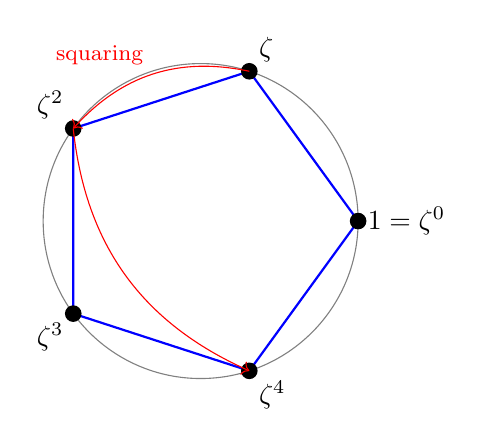
\begin{tikzpicture}[scale=2]
    % Circle
    \draw[gray, thin] (0,0) circle (1cm);
    
    % Vertices of the Pentagon
    \foreach \i in {0,1,2,3,4} {
        \coordinate (P\i) at ({cos(72*\i)}, {sin(72*\i)});
    }
    
    % Draw Pentagon
    \draw[thick, blue] (P0) -- (P1) -- (P2) -- (P3) -- (P4) -- cycle;
    
    % Nodes
    \fill[black] (P0) circle (1.5pt) node[right] {$1 = \zeta^0$};
    \fill[black] (P1) circle (1.5pt) node[above right] {$\zeta$};
    \fill[black] (P2) circle (1.5pt) node[above left] {$\zeta^2$};
    \fill[black] (P3) circle (1.5pt) node[below left] {$\zeta^3$};
    \fill[black] (P4) circle (1.5pt) node[below right] {$\zeta^4$};
    
    % Arrow showing structure
    \draw[->, red, bend right] (P1) to node[auto, swap] {\footnotesize squaring} (P2);
    \draw[->, red, bend right] (P2) to (P4);
    
\end{tikzpicture}
\captionof{figure}{The "Rigid" Structure. The roots form a regular pentagon. More importantly, they are powers of each other. If you move $\zeta$, you drag $\zeta^2$ (which is $\zeta \cdot \zeta$) with it.}
\end{center}

\subsubsection*{Why can't we just swap any two roots?}
Suppose we try to construct a permutation $\tau$ that swaps $\zeta$ and $\zeta^2$ but leaves $\zeta^3$ fixed.
\[ \tau(\zeta) = \zeta^2, \quad \tau(\zeta^2) = \zeta, \quad \tau(\zeta^3) = \zeta^3 \]
This is a valid permutation of the set $R$. However, let us check if it is a valid field automorphism.

In the field, $\zeta^2$ is algebraically related to $\zeta$ by the squaring operation:
\[ \zeta^2 = \zeta \cdot \zeta \]
A valid automorphism $\tau$ must respect this multiplication:
\[ \tau(\zeta^2) = \tau(\zeta \cdot \zeta) = \tau(\zeta) \cdot \tau(\zeta) \]
Substitute our proposed values:
\[ \text{LHS: } \tau(\zeta^2) = \zeta \]
\[ \text{RHS: } \tau(\zeta) \cdot \tau(\zeta) = \zeta^2 \cdot \zeta^2 = \zeta^4 \]
\[ \zeta \neq \zeta^4 \]

The relation is broken. The roots are ``locked'' together by the exponential relation. Once you decide where $\zeta$ goes, the destination of $\zeta^2, \zeta^3,$ and $\zeta^4$ is mathematically forced. This rigidity drastically reduces the size of the Galois group.

\subsection{Summary}
The Galois group measures the ``ambiguity'' of the roots relative to the base field.
\begin{itemize}
    \item It is the group of automorphisms of the splitting field that fix the base field.
    \item It is a subgroup of the permutations of the roots.
    \item It is the full symmetric group ($S_n$) only when there are no algebraic relations between the roots other than the polynomial equation itself.
\end{itemize}

\section{Closing: The Philosophy of Mathematical Structure}

Mathematics is often mischaracterized as the study of calculations. More accurately, it is the study of \textit{structures}. A mathematical structure is not merely a collection of objects; it is a rigorous "environment" or "landscape" defined by specific constraints.

Much of modern mathematics studies \emph{structures}: collections of objects equipped with specified operations and relations, constrained by axioms. The axioms are not mere restrictions; they are what make reasoning \emph{stable} and \emph{transportable} across contexts.


\begin{figure}[t]
    \centering
    \includegraphics[width=1\linewidth]{structure.png}
    \caption{A pedagogical illustration visualized as a chalkboard diagram, explaining the concept of mathematical structure in the context of a field extension, such as $L = \mathbb{Q}(i)$ over the base field $K = \mathbb{Q}$. The base field is depicted as a solid foundation, upon which a rigid framework of "Structural Constraints" (axioms and rules) is built, supporting the extended field $L$. This constrained environment ensures "Consistency," as shown by two different calculation paths (A and B) converging to the same result. The diagram also illustrates "Symmetry" (an automorphism) as a transformation that swaps indistinguishable roots while leaving the underlying structure invariant.}
    \label{fig:structure}
\end{figure}

\subsection{Structure as Constraint}
To build a structure is to impose rules. When we define a Group, a Ring, or a Field, we are essentially saying: "You cannot move arbitrarily; you must move according to these laws." 

Paradoxically, these constraints are what give mathematics its power. Because we are moving in a constrained world, we gain \textbf{consistency}.
\begin{itemize}
    \item \textbf{Path Independence:} In a structured world, if you start at point $A$ and apply valid operations to reach point $B$, the specific path you took often matters less than the rules you followed. 
    \item \textbf{Predictability:} If we calculate $(a+b)^2$ in the integers, or in the real numbers, or in a complex field, the result is always $a^2 + 2ab + b^2$. The \textit{structural rules} (distributivity and commutativity) guarantee this consistency across different contexts.
\end{itemize}

\begin{insight}
    \textbf{Structure ensures Semantic Consistency.} \\
    You can perform a calculation in different ways—grouping terms differently (associativity) or ordering them differently (commutativity)—and arrive at the exact same endpoint. This is only possible because the structure is "rigid." It holds its shape under calculation. \\

    Axioms license rewrites (rebracketing, expansion, reordering when permitted) that preserve denotation. “Different-looking” derivations converge because they are constrained by the same invariants.
\end{insight}

\subsection{Extending Structures: The Case of $\mathbb{Q}(i)$}

This perspective is crucial when we discuss \textbf{field extensions}. When we extend a field, we are expanding our "landscape," but we demand that the new landscape respects the structural integrity of the old one.

Consider the extension of the rational numbers $\Q$ by the imaginary unit $i$, denoted as $\Q(i)$.
\[
    \Q(i) = \{ a + bi \mid a, b \in \Q \}
\]
We are not simply throwing $i$ into a bag with rational numbers. We are forcing $i$ to submit to the pre-existing arithmetic structure of $\Q$.
\begin{itemize}
    \item We demand that multiplication remains distributive.
    \item We demand that addition remains commutative.
\end{itemize}

Because of these constraints, the behavior of every new element is pre-determined. For example, the product of $(1+i)$ and $(1-i)$ is not arbitrary; the structure forces it to be $2$. The "grid" of numbers has expanded, but the "lines of logic" connecting them remain straight and unbroken.

\subsection{From Structure to Symmetry}

Finally, structure gives rise to \textit{symmetry}. In a purely chaotic set with no structure, "symmetry" is meaningless because there is no shape to preserve. Symmetry is, by definition, a transformation that leaves the underlying structure invariant.

In our example of $\Q(i)$, the structure is defined by the rational numbers and the property that $i^2 = -1$. 
\begin{itemize}
    \item Notice that $(-i)^2 = -1$ as well.
    \item From the perspective of the structure $\Q$, the elements $i$ and $-i$ are indistinguishable. They play the exact same structural role.
\end{itemize}

This structural ambiguity allows us to swap $i$ and $-i$ without breaking the arithmetic. This swap is a \textbf{symmetry} (specifically, an automorphism). 




Structure thus gives rise to \emph{symmetry} in the precise sense of \emph{structure-preserving maps}. In field theory, the relevant symmetries are \textbf{field automorphisms} that fix the base field pointwise.

% In $\mathbb{Q}(i)/\mathbb{Q}$, an automorphism $\sigma$ must fix every rational number, and it must send $i$ to another element satisfying the same defining constraints. Concretely, $i$ is a root of its minimal polynomial over $\mathbb{Q}$,
% \[
% x^2+1,
% \]
% so any $\mathbb{Q}$-automorphism must send $i$ to another root of $x^2+1$, i.e., to $i$ or $-i$. Thus there are exactly two symmetries:
% \[
% \sigma(i)=i \quad\text{or}\quad \sigma(i)=-i,
% \]
% giving $\mathrm{Gal}(\mathbb{Q}(i)/\mathbb{Q})\cong C_2$.

\begin{insight}
    \textbf{Symmetry is the Shadow of Structure.} \\
    The more rigid and constrained the structure, the more meaningful the symmetries become. In Galois Theory, we study field extensions by analyzing these symmetries. We ask: "What are the ways we can move around inside this structure without breaking the rules?" \\

    Automorphisms are precisely the self-maps that preserve all axioms and defining relations. Studying an extension via its automorphisms is the core move of Galois theory: classify what can change without breaking the rules.
\end{insight}





\section{Algorithmic Structure and Galois Symmetry: the Example of $\mathbb{Q}(i)$}
\label{sec:ait-galois-qi}

A useful way to connect \emph{algorithmic information} (AIT) and \emph{Galois theory} is to treat a mathematical structure as something generated by a concise specification (a ``short program''), and to view \emph{symmetry} as the residual ambiguity left once the specification has fixed all invariants it can.

\subsection{A short generative description of the extension}
The field $\mathbb{Q}(i)$ can be defined by a minimal algorithmic specification:
\begin{quote}
Start with $\mathbb{Q}$ and adjoin an element $x$ subject to the single constraint $x^2+1=0$.
\end{quote}
Formally, this construction is captured by the quotient
\begin{equation}
\mathbb{Q}(i)\ \cong\ \mathbb{Q}[x]/(x^2+1),
\label{eq:Qi-quotient}
\end{equation}
where the coset $[x]$ plays the role of $i$, and every element has a unique representative $a+bx$ with $a,b\in\mathbb{Q}$ (reduction modulo $x^2+1$). This is a standard instance of the general fact that adjoining an algebraic element $\alpha$ with minimal polynomial $m_\alpha(x)$ yields an isomorphic field $F(\alpha)\cong F[x]/(m_\alpha(x))$ \cite{MilneFT,ArtinGalois71}.

From an AIT/MDL viewpoint, Eq.~\eqref{eq:Qi-quotient} emphasizes that the extension is specified by a \emph{small description}: ``the base field $\mathbb{Q}$, plus a single polynomial constraint $x^2+1=0$, plus the canonical quotient construction.'' In this sense, the \emph{regularity} defining $\mathbb{Q}(i)$ is precisely what makes the structure compressible in the Kolmogorov/MDL sense \cite{Kolmogorov65,Rissanen78}.


\begin{figure} [t]
    \centering
    \includegraphics[width=1\linewidth]{compression.png}
    \caption{\textbf{The Algorithmic Origins of Symmetry.} 
This diagram illustrates the synthesis of Algorithmic Information Theory (AIT) and Galois Theory using the extension $\mathbb{Q}(i)$. 
\textbf{(Left)} The minimal polynomial $P(x) = x^2+1$ is viewed as a "generating program" with low Kolmogorov complexity. This short code completely describes the structure of the extension. 
\textbf{(Center)} Because the program specifies a relationship ($x^2 = -1$) rather than unique identities, it leads to "algorithmic indistinguishability" between the solutions.
\textbf{(Right)} This indistinguishability manifests as a symmetry (automorphism) in the complex plane, where swapping the roots $i$ and $-i$ leaves the underlying algorithmic structure invariant.}
    \label{fig:compression}
\end{figure}

\subsection{Symmetry as residual ambiguity compatible with the specification}
Once the extension is fixed by its defining constraint, the admissible symmetries are exactly those transformations that preserve \emph{all} structure---i.e., field automorphisms fixing the base field pointwise. In $\mathbb{Q}(i)/\mathbb{Q}$, any $\sigma\in\mathrm{Gal}(\mathbb{Q}(i)/\mathbb{Q})$ must fix $\mathbb{Q}$ and send $i$ to another element satisfying the same minimal polynomial $x^2+1$. Since the roots are $\{i,-i\}$, there are exactly two possibilities:
\begin{equation}
\sigma(i)=i\quad\text{or}\quad \sigma(i)=-i,
\end{equation}
so
\begin{equation}
\mathrm{Gal}(\mathbb{Q}(i)/\mathbb{Q})\ \cong\ C_2.
\label{eq:gal-qi}
\end{equation}
Thus, the sole nontrivial symmetry is the swap $i\mapsto -i$ (complex conjugation restricted to $\mathbb{Q}(i)$) \cite{ArtinGalois71,MilneFT}.

\subsection{An AIT reading: ``one bit'' of unresolved choice}
The defining ``program'' for $\mathbb{Q}(i)$ specifies the extension \emph{up to} the choice of which root is named as the generator: the constraint $x^2+1=0$ does not distinguish $i$ from $-i$. This leftover indistinguishability is exactly the Galois symmetry in Eq.~\eqref{eq:gal-qi}. In this toy example, the size of the symmetry group corresponds to a literal ``one-bit'' ambiguity:
\begin{equation}
\log_2 \big|\mathrm{Gal}(\mathbb{Q}(i)/\mathbb{Q})\big|=\log_2 2=1.
\end{equation}
Interpretationally: given the concise generative description (Eq.~\eqref{eq:Qi-quotient}), specifying a particular identification of the adjoined element requires one additional bit (choose the $+$ or $-$ root). In this sense, \emph{Galois symmetry measures the degrees of freedom that remain after the structural constraints have fixed all invariants they can}.

\paragraph{Takeaway.}
Structure can be viewed as a compressive, algorithmic specification (constraints + canonical construction), while symmetry is the ``shadow'' of that specification: the transformations that preserve all constraints, equivalently the residual ambiguity not resolved by the description. The extension $\mathbb{Q}(i)/\mathbb{Q}$ provides a minimal illustration: a short description generates the structure, and the single surviving ambiguity manifests as the nontrivial Galois automorphism $i\mapsto -i$.




% ==========================================
% PART 2
% ==========================================
\clearpage
\part{Solvability, Complexity, and The Algorithmic Agent}
 
\section{The Solvability of Equations: From Geometry to Algebra}

We have established that the Galois group encodes the symmetry of an equation's roots. But why do we care about this symmetry? The historical triumph of Galois theory was not just in defining these groups, but in using them to determine which mathematical problems are \textit{possible} to solve.

We can classify numbers based on the tools required to generate them. This classification reveals a strict hierarchy, shown in Figure~\ref{fig:hierarchy}.

\begin{figure}[h]
    \centering
    % Placeholder for the first image generated (Hierarchy of Numbers)
    \includegraphics[width=0.85\linewidth]{hierarchy.png}

    
    \caption{\textbf{The Hierarchy of Numbers.} Note the distinction between Algebraic numbers (roots of polynomials) and the subset of those that are Expressible by Radicals. Transcendental numbers (like $\pi$) live entirely outside the algebraic realm.}
    \label{fig:hierarchy}
\end{figure}

 



\subsection{Constructible vs. Expressible: The Geometric Gap}

A common point of confusion is the difference between numbers that can be "constructed" and those that can be "written as a formula." These are distinct concepts based on the "hardware" allowed:

\begin{enumerate}
    \item \textbf{Constructible Numbers (Ruler \& Compass):} Ancient Greek geometry allows only two operations: drawing a line through two points and drawing a circle. Algebraically, finding the intersection of lines and circles corresponds to solving \textbf{linear} and \textbf{quadratic} equations. Therefore, a number is constructible only if it can be built using integers and \textbf{square roots} ($\sqrt{\cdot}$).
    \item \textbf{Expressible by Radicals:} Algebraic solvability allows a powerful upgrade. We are allowed to use \textit{any} $n$-th root ($\sqrt[3]{\cdot}, \sqrt[4]{\cdot}, \sqrt[5]{\cdot}$, etc.).
\end{enumerate}

\begin{figure}[t]
    \centering
    % Placeholder for the distinction image (Expressible vs Constructible)
    \includegraphics[width=1\linewidth]{constructible.png}
    \caption{\textbf{Tools Determine the Domain.} Constructible numbers are limited to square roots because the intersection of circles and lines never yields a degree higher than 2. "Doubling the Cube" requires $\sqrt[3]{2}$, which is expressible by radicals but impossible to construct with a compass.}
    \label{fig:constructible}
\end{figure}

 

This distinction solves the ancient problem of \textbf{Doubling the Cube}. To double a cube of volume 1, we need a side length of $\sqrt[3]{2}$.
\begin{itemize}
    \item Is $\sqrt[3]{2}$ expressible by radicals? \textbf{Yes.} (We just wrote it).
    \item Is $\sqrt[3]{2}$ constructible? \textbf{No.} The Galois group of $x^3-2$ implies a degree of 3. Constructible operations only allow degrees that are powers of 2 (compounded square roots).
\end{itemize}

\subsection{The General Solvability Condition}

The most profound result of the theory is the criterion for solvability by radicals. Can we find a formula for the roots of a polynomial using only $+,-,\times,\div$ and $\sqrt[n]{\cdot}$?

Galois proved that an equation is solvable if and only if its Galois group is "Solvable."

\begin{definition}[Solvable Group (Informal)]
    A group $G$ is solvable if it can be broken down into a series of "simple" abelian layers. Effectively, this means the complex symmetry can be decomposed into a sequence of prime-order cyclic steps, each corresponding to extracting an $n$-th root.
\end{definition}

For polynomials of degree $n \leq 4$, the symmetric group $S_n$ is solvable. This is why we have the Quadratic Formula, the Cubic Formula, and the Quartic Formula.

However, for $n = 5$, the symmetric group $S_5$ is \textbf{not solvable}. It contains symmetries so tangled that they cannot be untied into abelian steps. Consequently, there is no general formula for the Quintic equation.

\begin{figure}[h]
    \centering
    % Placeholder for the flowchart image (Solvability Logic)
    \includegraphics[width=0.95\linewidth]{solvability_flowchart.png}
    \caption{\textbf{The Galois Filter.} To determine if an equation is solvable, we analyze its Galois Group $G$. If $G$ is a "Solvable Group" (a specific group-theoretic property), we can derive a formula. If $G$ is not solvable (like $S_5$), the roots exist but cannot be expressed using radicals.}
    \label{fig:solvability}
\end{figure}

 

\begin{insight}
    \textbf{Symmetry as a barrier to calculation.} \\
    %We often think of symmetry as %something that makes problems easier (e.g., simplifying a physics problem). In Galois theory, \textit{too much} symmetry makes a problem impossible. \\

    If the permutations of the roots are maximally complex (the group $S_5$ or $A_5$), the structure is too "rigidly chaotic" to be broken down. We cannot isolate the roots one by one using radicals because the group structure refuses to be dismantled.
\end{insight}


\subsection{The Meaning of "Solvable": Compositionality vs. Chaos}

Why does the structure of a group determine if we can write a formula? The key lies in \textbf{decomposition}.

A formula like the Quadratic Formula is essentially a sequential computer program:
\begin{enumerate}
    \item Calculate the discriminant $D$.
    \item Take a square root (Step 1).
    \item Perform arithmetic to find $x$ (Step 2).
\end{enumerate}

This step-by-step approach works only because the symmetry group of the quadratic equation can be broken down into smaller, independent layers (subgroups). We solve the symmetry "one layer at a time."

\begin{itemize}
    \item \textbf{Solvable Groups (Compositional):} These groups have a hierarchical structure. They can be factored into a "tower" of simple abelian groups. This algebraic decomposition corresponds exactly to the algorithmic process of taking successive $n$-th roots.
    \item \textbf{Unsolvable Groups (Monolithic):} The group of the general Quintic equation ($S_5$) contains a massive, "atomic" core called a \textit{Simple Group} ($A_5$). This structure has no internal layers—it is a solid block of symmetry that cannot be factored.
\end{itemize}


\begin{figure}[t]
    \centering
    \includegraphics[width=1\linewidth]{compositionality.png}
    \caption{Compositionality and Solvability}
    \label{fig:placeholder}
\end{figure}
\begin{insight}
    \textbf{Solvability is Decomposability.} \\
    
    Your intuition is correct: a "solvable" problem is one that is \textbf{compositional}. It can be broken down into a sequence of simpler problems (abelian extensions). \\
    
    The "Unsolvable" Quintic is not unsolvable because it lacks symmetry, but because its symmetry is \textbf{monolithic}. It acts like a "Gordian Knot"—a tangled mess of dependencies that cannot be untied strand by strand. Because the Group cannot be decomposed into steps, the solution cannot be written as a step-by-step formula (radicals).
\end{insight}




\section{Beyond Radicals: The Nuclear Option}

The Abel-Ruffini theorem places a hard limit on what we can do with our standard toolbox. It proves that the "lock" of the Quintic equation ($S_5$) is too complex for the "key" of standard radicals ($\sqrt[n]{\cdot}$).

However, in mathematics, if a problem is impossible, we often simply invent new tools. "Unsolvable" does not mean the number doesn't exist; it just means we need a more sophisticated function to name it.

\subsection{The ``Bring Radical": A Specific Key}
In 1786, Erland Bring proved that any quintic equation can be transformed (using standard algebra) into a highly simplified "normal form":
\[ x^5 + x + a = 0 \]
The obstruction here is the linear term $+x$. Standard roots cannot invert the sum of two different powers. To solve this, mathematicians effectively created a "Quintic Root" button. We define the \textbf{Bring Radical}, denoted $BR(a)$, as the real root of this specific equation.
With this expanded toolkit ($\sqrt[n]{\cdot}$ plus $BR(\cdot)$), \textit{all} quintic equations become solvable!

\subsection{The ``Nuclear Option": Elliptic Functions}
A far deeper solution comes from geometry.
\begin{itemize}
    \item \textbf{Standard Roots ($\sqrt[n]{}$)} are related to the geometry of the \textbf{Circle} (cyclic groups).
    \item \textbf{The Quintic ($S_5$)} is related to the geometry of the \textbf{Icosahedron}.
\end{itemize}

The symmetry group of the Icosahedron is isomorphic to $A_5$ (the rigid core of the quintic). Because standard roots correspond to circles, they cannot map onto the icosahedral structure.

In 1858, Hermite and Kronecker proved that \textbf{Elliptic Modular Functions}—complex functions used to study elliptic curves—possess exactly the right internal symmetries to "unlock" the Quintic. Just as trigonometric functions ($\sin, \cos$) solve problems involving circles, modular functions solve problems involving icosahedral symmetry.

\begin{figure}[t]
    \centering
    \includegraphics[width=0.95\linewidth]{nuclear_option.png}
    \caption{\textbf{Matching the Tool to the Symmetry.} The "Lock" of the Quintic equation is the non-abelian group $A_5$ (isomorphic to the Icosahedron). Standard radicals (Cycle) are too simple to unlock it. We need Modular Functions, which possess the requisite Icosahedral symmetry.}
    \label{fig:nuclear}
\end{figure}


 

\begin{insight}
    \textbf{Symmetry Matching.} \\
    The solvability of an equation comes down to a matching game. To write a formula for a number, the "Symmetry of the Tool" must be compatible with the "Symmetry of the Equation." \\

    Radicals have \textit{Abelian} (commutative) symmetry. They fail on the Quintic because the Quintic has \textit{Non-Abelian} symmetry. By upgrading to Elliptic functions (which handle non-abelian transformations), the "unsolvable" becomes solvable.
\end{insight}



\section{The Continuous Frontier: Compositionality in Calculus and Learning}

The story of solvability does not end with polynomials. In the late 19th century, Sophus Lie asked a profound question: \textit{Can we build a Galois Theory for Differential Equations?}

Just as we ask if a polynomial allows a step-by-step formula using radicals, we can ask if a differential equation allows a step-by-step solution using \textbf{integrals} (quadratures).

This line of inquiry leads us directly to modern learning theory. The mathematical condition that makes an equation "solvable" is identical to the structural condition that makes a complex environment "learnable" by an algorithmic agent.

\subsection{Differential Galois Theory: Integration as Decomposition}
For a differential equation, the symmetries of the solution space form a \textbf{Lie Group} (or, in the infinite case, a Lie Pseudogroup).
\begin{itemize}
    \item \textbf{Solvable (Compositional):} If this group decomposes into a "tower" of abelian subgroups, the equation is solvable. We can build the solution by stacking integrals one on top of another.
    \item \textbf{Monolithic (Not Solvable):} If the group is "simple" (like $SL_2(\mathbb{C})$ in the Airy equation), the symmetry is a solid block. The solution cannot be broken down into elementary steps; it defines a new, irreducible "atomic" complexity.
\end{itemize}

Sophus Lie proved that if a differential equation admits a Solvable Lie group of symmetries, we can perform a \textbf{reduction of order}:
\[ \text{Order } n \xrightarrow{\text{Symmetry } 1} \text{Order } n-1 \xrightarrow{\dots} \text{Integration} \]
The "Solvability" of the group literally measures whether the system can be dismantled step-by-step.

\subsection{The Unifying Thread: From Galois to Poggio and Ruffini}

This algebraic hierarchy mirrors the fundamental constraints of intelligence and learning.

\paragraph{Poggio and the Curse of Dimensionality.}
Tomaso Poggio and colleagues have shown that the effectiveness of Deep Neural Networks hinges on \textbf{Compositionality} \cite{PoggioMhaskar17}. Generic functions suffer from the "Curse of Dimensionality"—learning them requires exponentially many samples. However, functions that describe the physical world are rarely generic; they are \textit{compositional} (hierarchical and local).
Just as a solvable Galois group decomposes into a tower of simple extensions, a learnable function decomposes into a tower of simple constituent functions:
\[ F(x) = f_L(f_{L-1}(\dots f_1(x)\dots)) \]
Deep networks succeed because their architecture matches this solvable structure. They are the "Abelian towers" of function approximation.

\paragraph{Structured Dynamics in the Algorithmic Agent.}
This connects directly to the framework of \textbf{Structured Dynamics} proposed in \cite{Ruffini24}. An algorithmic agent is not a passive observer but an active solver. For an agent to efficiently predict or control its environment, the "symmetry group" of the environment's dynamics must be solvable relative to the agent's computational resources.

If the environment is "monolithic" (lacking decomposable symmetries), the agent faces an irreducible wall of algorithmic complexity. Intelligence, therefore, is the ability to identify and exploit the \textit{reduction of order} permitted by the symmetries of the world.

\begin{figure}[t]
    \centering
    \includegraphics[width=1\linewidth]{continuous.png}
    \caption{\textbf{The Universal Logic of Solvability.} This diagram illustrates the structural parallel between Galois Theory, Differential Equations, and Learning Theory. In all domains, "solvability" is equivalent to \textbf{Decomposability}. A problem is tractable only if its complexity can be factorized into a "tower" of atomic operations—whether those are roots, integrals, or neural network layers. If the underlying symmetry group is monolithic (like $A_5$), the step-by-step construction fails, representing a barrier to both symbolic solution and efficient learning.}
    \label{fig:solvability_universal}
\end{figure}

\begin{figure} [t]
    \centering
    \includegraphics[width=1\linewidth]{continuous2.png}
    \caption{\textbf{The Universal Logic of Tractability.}
This infographic synthesizes the parallel constraints across three domains.
\textbf{(Left \& Center)} In mathematics, a problem is "solvable" (by radicals or integrals) only if its symmetry group is \textit{compositional}—meaning it can be decomposed into a "tower" of elementary abelian steps. If the group is monolithic (simple), the step-by-step derivation fails.
\textbf{(Right)} This same principle governs Artificial Intelligence. As shown by Poggio and Mhaskar, and formalized in the \textit{Structured Dynamics} framework (Ruffini 2024), efficient learning is only possible when the environment's complexity is hierarchical (compositional). A "monolithic" environment, lacking this structure, succumbs to the Curse of Dimensionality, rendering it effectively "unsolvable" for an algorithmic agent.}
    \label{fig:placeholder}
\end{figure}

\begin{insight}
    \textbf{Compositionality is Universal.} \\
    Whether in Algebra, Calculus, or AI, "Solvability" always means the same thing: \textbf{Decomposability.}

    \begin{itemize}
        \item \textbf{Algebra:} A Solvable Group lets us build a number by composing roots: $\sqrt{2 + \sqrt{3}}$.
        \item \textbf{Calculus:} A Solvable Lie Group lets us build a function by composing integrals: $y(x) = \int e^{\int f(t) dt} dx$.
        \item \textbf{Learning:} A Compositional Function class lets us approximate reality with polynomial (rather than exponential) sample complexity \cite{PoggioMhaskar17}.
    \end{itemize}
    
    As argued in \cite{Ruffini24}, this is the core constraint of the Algorithmic Agent. We can only ``solve" (or efficiently model) that which is structured. A ``monolithic" symmetry group corresponds to maximum algorithmic entropy—a structure that resists compression into a sequence of steps.
\end{insight}

\section{The Algorithmic Staircase: Composition, Discovery, and Re-Composition}

In the framework of Algorithmic Information Theory (AIT), learning is the compression of the environment's dynamics. As noted in \cite{Ruffini17, Ruffini2022, Ruffini24}, the progress of an intelligent agent is best visualized via the \textbf{Kolmogorov Structure Function}, where the $y$-axis represents the remaining \textbf{Error} (uncertainty) and the $x$-axis represents the allowed \textbf{Model Complexity} (program length).

This function does not descend smoothly; it forms a \textbf{Staircase}. This shape reveals that intelligence oscillates between two distinct modes: standard optimization and structural discovery.

\subsection{Phase 1: Compositional Search (The Slope)}
Initially, the agent operates within a fixed language (e.g., standard arithmetic or a fixed neural architecture). It navigates the combinatorics of these tools to find the best fit for the data.
\begin{itemize}
    \item \textbf{Mechanism:} Rearranging existing primitives ($+,-,\times, \sqrt{}$) to minimize error.
    \item \textbf{Mathematical Analog:} Solving a polynomial by radicals. The specific \textit{arrangement} must be found, but the tools are constant.
    \item \textbf{The Barrier:} Eventually, this process hits the "Monolithic Barrier" (an ignorance plateau). If the phenomenon has a symmetry not present in the toolkit (like the $A_5$ core of the Quintic), simple composition stalls.
\end{itemize}

\subsection{Phase 2: Primitive Discovery (The Drop)}
This is the "Nuclear Option." To breach the barrier, the agent must expand its language by identifying a rigid, non-decomposable sub-structure and "compiling" it into a new atomic symbol.
\begin{itemize}
    \item \textbf{Mechanism:} Identifying a recurring pattern (e.g., translation invariance) and evolving a new \textbf{Cognitive Core} (e.g., a Convolutional layer).
    \item \textbf{Mathematical Analog:} Defining the \textbf{Bring Radical} or the \textbf{Airy Function}.
    \item \textbf{Result:} A massive, "vertical" drop in the structure function. A small investment in complexity (defining the new symbol) yields a huge reduction in error.
\end{itemize}

\begin{figure}[t]
    \centering
    \includegraphics[width=1\linewidth]{staircase.png}
    \caption{\textbf{The Staircase of Understanding.}
    The Kolmogorov Structure Function ($K(M)$ vs. Error $\epsilon$) descends in steps.
    \textbf{(1) Composition:} The agent optimizes using current tools.
    \textbf{(2) Discovery:} The agent hits a "Monolithic Barrier." Discovering a new Cognitive Core (e.g., a CNN or Special Function) triggers a sharp drop.
    \textbf{(3) Re-Composition:} The agent now optimizes using the expanded toolkit, continuing the cycle.}
    \label{fig:staircase}
\end{figure}


\subsection{Phase 3: Re-Composition (The New Slope)}
Crucially, the process does not stop at discovery. Once the new primitive is added to the library, \textbf{compositionality is expanded}. The agent enters "Compositional Search 2.0," optimizing combinations of the \textit{new} tool with the \textit{old} ones. The error curve begins to descend again, exploring a deeper valley of solvability.

This cycle is not merely a heuristic; it is a fundamental requirement for any system trying to model our specific physical reality. As Tomaso Poggio argues in his upcoming lectures, the success of these systems mirrors the structure of the universe itself:

\begin{quote}
    ``Modern deep learning works astonishingly well, yet we still lack a fundamental understanding of \textit{why}. [...] It is a natural phenomenon that demands explanation in terms of underlying principles. [...] Two principles emerge repeatedly: \textbf{(sparse) compositionality} and \textbf{genericity}. [...] They are not heuristic conjectures, but logical inevitabilities derived from the foundations of computation and physics.'' \cite{Poggio26}
\end{quote}

The "Staircase" is simply the algorithmic manifestation of this sparse compositionality.



\begin{insight}
    \textbf{The Cycle of Intelligence (Compression).} \\
    Intelligence is not just finding one formula; it is a cycle of \textbf{Defining} new primitives and \textbf{Composing} them.
    \[ \text{Compose} \xrightarrow{\text{Stall}} \text{Discover Primitive} \xrightarrow{\text{Expand}} \text{Re-Compose} \rightarrow \dots \]
    Galois Theory teaches us that "Solvability" is the easy part (Composition). The history of mathematics—and AI—is defined by the hard part: discovering the new primitives that make the unsolvable solvable again.
\end{insight}

\clearpage
%%%%%%%%%%%%%%%%
% --- Bibitems for the AIT–Galois section ---
\begin{thebibliography}{99}
\bibitem{MilneFT}
J.~S.~Milne,
\newblock \emph{Fields and Galois Theory} (course notes, v4.60, Sept.~2018).
\newblock Available at:
\href{https://www.jmilne.org/math/CourseNotes/FT.pdf}{https://www.jmilne.org/math/CourseNotes/FT.pdf}.

\bibitem{ArtinGalois71}
E.~Artin,
\newblock \emph{Galois Theory: Lectures Delivered at the University of Notre Dame} (rev. ed.),
\newblock edited by A.~N.~Milgram, Notre Dame Mathematical Lectures, No.~2, 1971.
\newblock Available at:
\href{https://projecteuclid.org/ebooks/notre-dame-mathematical-lectures/Galois-Theory/toc/ndml/1175197041}{Project Euclid (NDML)}.

\bibitem{Kolmogorov65}
A.~N.~Kolmogorov,
\newblock ``Three approaches to the definition of the concept `quantity of information',''
\newblock \emph{Problemy Peredachi Informatsii} \textbf{1}(1): 3--11, 1965.
\newblock Accessible PDF:
\href{https://alexander.shen.free.fr/library/Kolmogorov65_Three-Approaches-to-Information.pdf}{https://alexander.shen.free.fr/library/Kolmogorov65\_Three-Approaches-to-Information.pdf}.
\newblock (Reprint/translation: \emph{International Journal of Computer Mathematics} \textbf{2}(1--4): 157--168, 1968,
DOI \href{https://doi.org/10.1080/00207166808803030}{10.1080/00207166808803030}.)

\bibitem{Rissanen78}
J.~Rissanen,
\newblock ``Modeling by shortest data description,''
\newblock \emph{Automatica} \textbf{14}(5): 465--471, 1978.
\newblock DOI \href{https://doi.org/10.1016/0005-1098(78)90005-5}{10.1016/0005-1098(78)90005-5}.

\bibitem{Ruffini24}
G.~Ruffini,
\newblock ``Structured Dynamics in the Algorithmic Agent,''
\newblock \emph{Preprint/Technical Note}, 2024.

\bibitem{PoggioMhaskar17}
T.~Poggio and H.~Mhaskar,
\newblock ``Why and when can deep-but not shallow-networks avoid the curse of dimensionality: A review,''
\newblock \emph{International Journal of Automation and Computing}, \textbf{14}(5): 503--519, 2017.
\newblock DOI \href{https://doi.org/10.1007/s11633-017-1054-2}{10.1007/s11633-017-1054-2}.

\bibitem{Ruffini17}
G.~Ruffini,
\newblock ``An Algorithmic Information Theory of Consciousness,''
\newblock \emph{Neuroscience of Consciousness}, \textbf{3}(1), 2017.
\newblock DOI \href{https://doi.org/10.1093/nc/nix019}{10.1093/nc/nix019}.

\bibitem{Ruffini22}
G.~Ruffini and E.~Lopez-Sola,
\newblock ``AIT Foundations of Structured Experience,''
\newblock \emph{Journal of Artificial Intelligence and Consciousness}, \textbf{9}(2): 153--191, 2022.
\newblock DOI \href{https://doi.org/10.1142/S2705078522500047}{10.1142/S2705078522500047}.

\bibitem{Poggio26}
T.~Poggio,
\newblock \emph{Thirty Brief Lectures on Foundations of Deep Learning} (Draft),
\newblock January 26, 2026.


\end{thebibliography}


\end{document}
